\documentclass[UTF8, xcolor=table]{beamer}
%\usepackage{fontspec}
%\setsansfont{宋体}
\usepackage[BoldFont,SlantFont]{xeCJK}
%\setCJKmainfont[BoldFont={SimHei},ItalicFont={KaiTi}]{SimSun}
\setCJKmainfont[BoldFont={Adobe Heiti Std},ItalicFont={Adobe Kaiti Std}]{SimSun}

\usepackage{latexsym,amssymb,amsmath,amsbsy,amsopn,amstext,xcolor,multicol}
\usepackage{graphicx,wrapfig,fancybox}
\usepackage{pgf,pgfarrows,pgfnodes,pgfautomata,pgfheaps,pgfshade}
\usepackage{thubeamer}
%\usepackage[backend=bibtex,style=IEEE,sorting=none]{biblatex} % [参考文献格式](https://www.sharelatex.com/blog/2013/07/31/getting-started-with-biblatex.html)
\usepackage[backend=bibtex,sorting=none]{biblatex} % [参考文献格式](https://www.sharelatex.com/blog/2013/07/31/getting-started-with-biblatex.html) %mac IEEE not found
\usepackage{array}
\usepackage{bm}
\usepackage{caption}
\usepackage[caption=false]{subfig}
\usepackage{multirow}
\usepackage{booktabs}
\usepackage{tikz}
\usepackage{tikzscale}

\defbibheading{bibliography}[\bibname]{} %avoid printbibliography 自动生成目录
\addbibresource{ref/papers-bib-in-google.bib}
\addbibresource{ref/chinese-ref.bib}
%\setbeamertemplate{bibliography item}{\insertbiblabel} %将列表中默认的丑陋的icon 改成数字,或者下面这个也行
\setbeamertemplate{bibliography item}[text] % [ref](http://tex.stackexchange.com/questions/68080/beamer-bibliography-icon)
%\setbeamertemplate{footline}[frame number]{}

%\setframeofframes{of}

\usepackage{boxedminipage} %for: bvh border
\def\fourgraphicswidth{0.35} %0.3\textwidth

\usepackage{algorithm} %%format of the algorithm
\usepackage{algpseudocode}
\floatname{algorithm}{算法}
\renewcommand{\algorithmicrequire}{\textbf{输入:}} %%Use Input in the format of Algorithm
\renewcommand{\algorithmicensure}{\textbf{输出:}} %%UseOutput in the format of Algorithm
%\algrenewcommand{\algorithmiccomment}[1]{\hskip3em $\rightarrow$ #1}
\algrenewcommand{\algorithmiccomment}[1]{ $//$ #1}

\usepackage{listings}
\renewcommand\lstlistingname{代码}
\renewcommand\lstlistlistingname{代码}

\lstset{framexleftmargin=1.4em,
        xleftmargin=1.8em,
        basicstyle=\ttfamily\small,
        %frame=shadowbox, numberstyle=\tiny, breaklines=true,
        frame=single,
        numberstyle=\tiny, breaklines=true,
        keywordstyle=\color{blue!70}\bfseries,
        %commentstyle=\color{red!50!green!50!blue!50},
        rulesepcolor=\color{red!20!green!20!blue!20},
        numbers=none,fontadjust=true}
\lstdefinelanguage{shader}{morekeywords={uniform, layout, uniform, vec2, vec3, vec4, in, out, gl_Position, dot, flat, int ,float, gl_VertexID, xyz, w, x, y, z, location, version, sampler2DRect, bgr, gl_FragData, texture2DRect, gl_TexCoord,for,xy},morecomment=[l]{//}}

\begin{document}

\setbeamerfont{footnote}{size=\tiny}
\setbeamerfont{caption}{size=\scriptsize}
\setbeamertemplate{caption}[numbered]

\graphicspath{{figures/}}

\title{凸包围多面体生成算法及应用}
%\author{唐磊}
\author[唐磊]{(申请清华大学工学硕士学位论文答辩报告)\vskip 20pt学~~~~~~生:唐~~~~~磊~~~~~~~~\vskip 5pt 指导教师:雍~俊~海~教授}
\institute[清华大学~软件学院~CG~\&~CAD~研究所]{\small \vskip 38pt计算机辅助设计图形学与可视化研究所}
%\date{2015-06-07}
\date{\small \vskip -17pt二〇一五年六月}
%\date{\today}



\frame{
\vspace{-15mm}
\titlepage
\vspace{-43mm}
\begin{figure}[htbp]
  \begin{center}
	
\includegraphics[width=0.16\linewidth]{Tsinghua_University_Logo.eps}
  \end{center}
\end{figure}
%\beign{picture}(1,1)
%\put(6,8){
\includegraphics[width=0.15\linewidth]{Tsinghua_University_Logo.eps}}
%\end{picture}
}

  \section*{目录}
  \frame {
    \frametitle{\secname}
    \tableofcontents
  }

  \AtBeginSubsection[] {
  \frame<handout:0> {
  \frametitle{目录}
  \tableofcontents[current,currentsubsection]
    }
  }

  \section{引言}
  \frame
  {
    \frametitle{\secname~ }
    \begin{block}{凸包围体技术}
      在计算机图形学领域里的各种算法中发挥着重要作用,
      如优化渲染和建模过程,加速求交、碰撞检测等算法。
    \end{block}

    \begin{block}{碰撞检测问题}
   计算机图形学、虚拟现实等领域中的研究热点,
   是计算机模拟真实环境中不可或缺的技术,
   在物理仿真及游戏领域里应用十分广泛。
    \end{block}
  }

  \subsection{凸包围体}
  \frame{
  \frametitle{凸包围体的种类}
  \begin{figure}
  \hspace{-2.0em}
    \begin{minipage}{1.06\textwidth}
    \subfloat[\scriptsize AABB]
        {
           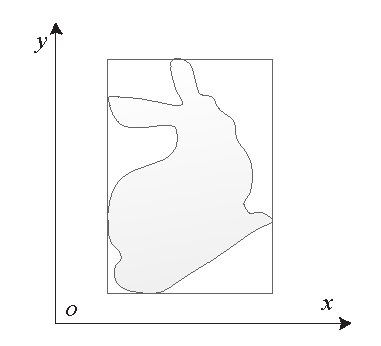
\includegraphics[width=0.2\textwidth]{figures/bunny-2d-AABB.eps}
        }
        \subfloat[\scriptsize OBB]
        {
            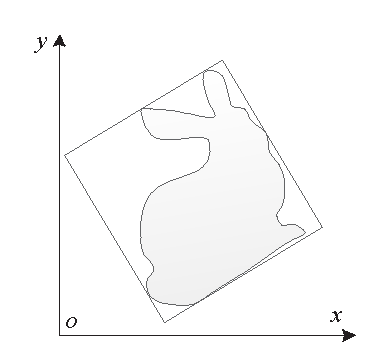
\includegraphics[width=0.2\textwidth]{figures/bunny-2d-OBB.eps}
        }
       \subfloat[\scriptsize Sphere]
        {
           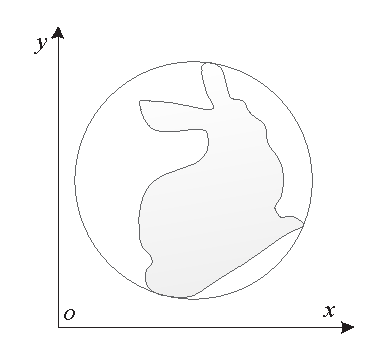
\includegraphics[width=0.2\textwidth]{figures/bunny-2d-Sphere.eps}
        }%\linebreak
        \subfloat[\scriptsize $k$-DOP]
        {
           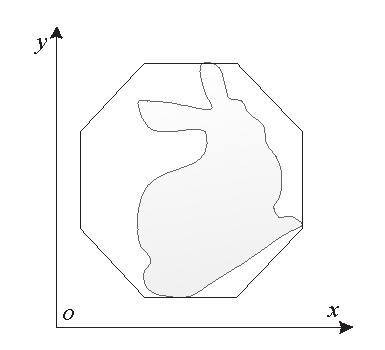
\includegraphics[width=0.2\textwidth]{figures/bunny-2d-8DOP.eps}
        }
        \subfloat[\scriptsize 凸包]
        {
           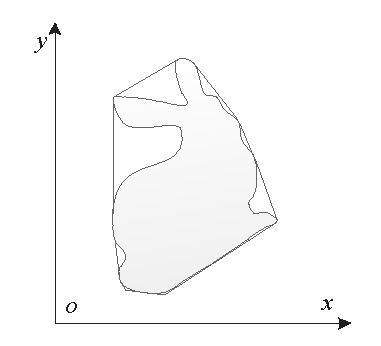
\includegraphics[width=0.2\textwidth]{figures/bunny-2d-Convexhull.eps}
        }
        \end{minipage}
        \caption{不同种类的包围体}
        \label{chart:exps:tightness}
        \end{figure}
        \vspace{-1em}
      其他:Tribox、Swept-sphere、 Sphere-shell、Zonotopes、圆柱形、圆锥、椭球形等等。
  }

      \frame{
   \frametitle{本文目标}
   \begin{block}{综合比较}
   \begin{description}
     \item[$k$-DOP\cite{klosowski1998efficient}:]方向固定且有限,不同模型其截面方向一致, 不够紧致。
     \item[凸包:]很(最)紧致, 但面片数量太多, 复杂度$O(n\log n)$。
    \end{description}
  \end{block}
  \begin{block}{本文凸包围体的目标}
     \begin{description}
     \item[紧致:] 能够自适应模型
     \item[快速:] 利用~GPU~加速
     \item[灵活:] 通过参数~$k$~调节简单性和紧致性
     \end{description}
   \end{block}
  }

  \subsection{碰撞检测算法}
   \frame{
   \frametitle{\subsecname~ }
    
   \begin{block}{碰撞检测算法}
    许多应用的基础,例如在~3D~游戏,物理仿真,机器人,虚拟现实等领域中。
   \end{block}

   \begin{block}{分类}
     \begin{description}
       \item[加速结构:] SPT(如四叉树、KD~树等)~v.s~\textbf{BVH}(OBB树、$k$-DOP树等)
       \item[表现形式:] \textbf{刚体}~v.s~可变形,凸体~v.s~凹体,CSG~v.s~参数曲面~v.s~\textbf{多边形网格}
       \item[碰撞环境:] \textbf{成对}~v.s~\textbf{多体},\textbf{静止}~v.s~\textbf{运动},\textbf{离散}~v.s~连续
     \end{description}
   \end{block}
  }

  \frame{
    \frametitle{基于~BVH~的碰撞检测算法}
    \begin{columns}[onlytextwidth]
      \begin{column}{0.35\textwidth}
        \vspace{-1.5em}
        \begin{figure}[htbp]
            \begin{center}
            \begin{boxedminipage}{1\textwidth}
            \subfloat{\label{lbl:bvh-bunny-center-0.png}}
              {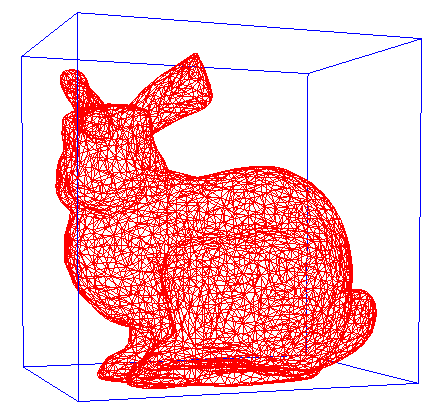
\includegraphics[height=1.4cm]{bvh-bunny-center-0.png}}
            \subfloat{\label{lbl:bvh-bunny-center-1.png}}
              {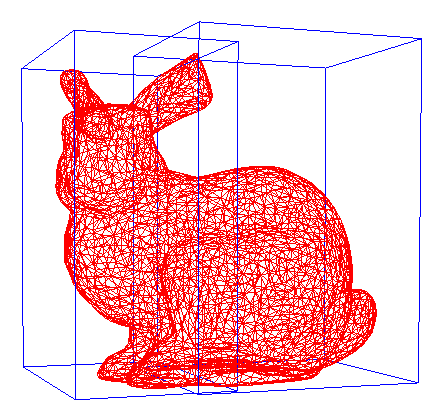
\includegraphics[height=1.4cm]{bvh-bunny-center-1.png}}
            \\
            \subfloat{\label{lbl:bvh-bunny-center-2.png}}
              {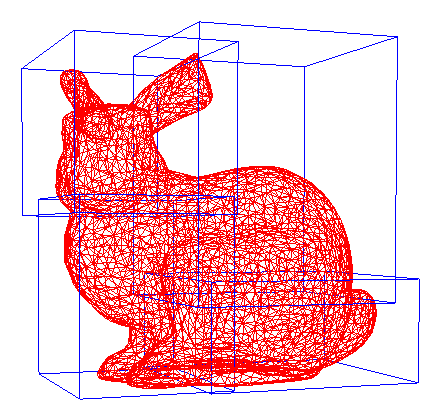
\includegraphics[height=1.4cm]{bvh-bunny-center-2.png}}
            \subfloat{\label{lbl:bvh-bunny-center-3.png}}
              {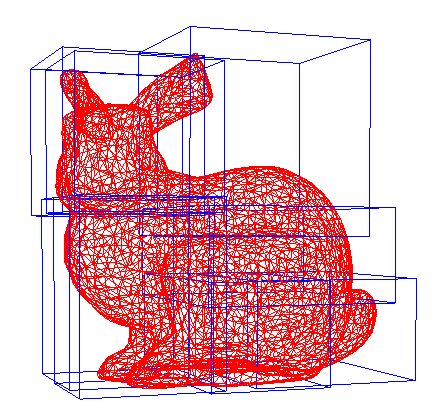
\includegraphics[height=1.4cm]{bvh-bunny-center-3.png}}
            \\\hspace{0.5cm}
            \subfloat{\label{lbl:bvh-bunny-center-4.png}}
              {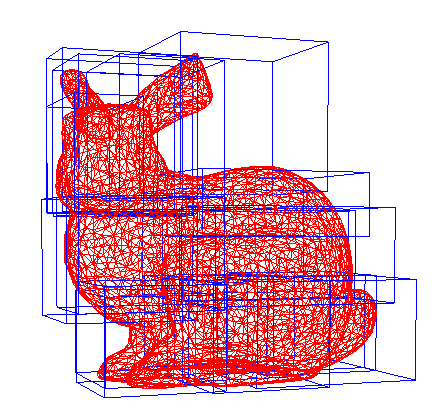
\includegraphics[height=1.5cm]{bvh-bunny-center-4.png}}
            \subfloat{\label{lbl:bvh-bunny-center-5.png}}
              {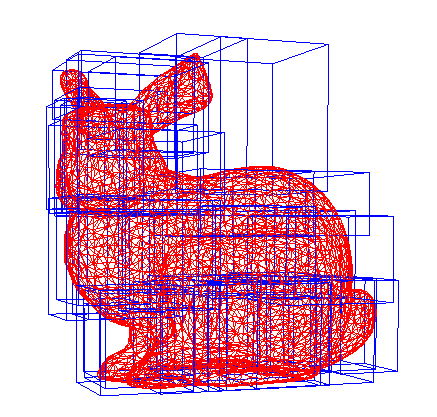
\includegraphics[height=1.5cm]{bvh-bunny-center-5.png}}
            \\
            \subfloat{\label{lbl:bvh-bunny-center-6.png}}
              {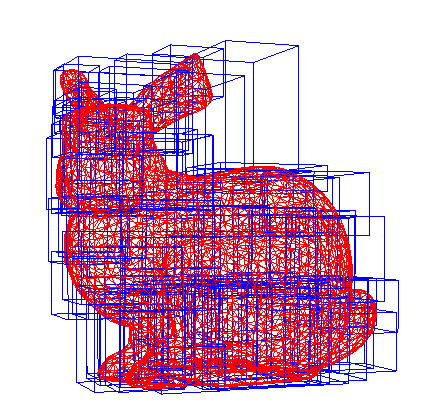
\includegraphics[height=1.5cm]{bvh-bunny-center-6.png}}
            \subfloat{\label{lbl:bvh-bunny-center-7.png}}
              {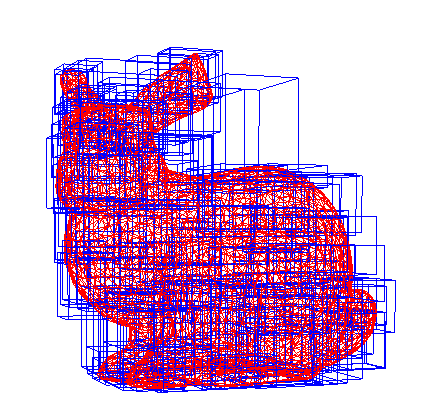
\includegraphics[height=1.5cm]{bvh-bunny-center-7.png}}
            \end{boxedminipage}
            \vspace{-0.5em}
          \caption{八层~BVH~示例}
          \label{lbl:bvh-example}
          \end{center}
          \end{figure}
      \end{column}
      \hspace{0.5em}
      \begin{column}{1.2\textwidth}
      \vspace{0.2em}
         \scalebox{0.5}{
              \begin{minipage}{1.0\textwidth}
      \vspace{-2em}
           \begin{algorithm}[H]
              \caption{自顶向下层次遍历~BVH~}
              \label{alg:traverse-bvh-tree}
              \begin{algorithmic}[1]
              \Require
              两个~BVH~树的根节点~$node_1$,$node_2$
              \Ensure
              模型是否相交
              \Function {TraverseBVHTree}{$node_1, node_2$}
                \If{$node_1.bv \cap node_2.bv = \emptyset$}
                  \State \Return{\textbf{False}}
                  \Comment{包围体重合测试, 包围体不相交直接返回}
                \Else
                    \If {$node_1.children = \emptyset$}
                         \If {$node_2.children = \emptyset$}
                         \State \Comment{最底层叶子节点原生几何相交测试}
                         \State \Return {\Call{CheckIntersection}{$node_1.primitives, node_2.primitives$}}
                         \Else
                            \ForAll {$child \in node_2.children$}
                            \State \Call{TraverseBVHTree}{$node_1, child$} \Comment{递归调用}
                            \EndFor
                         \EndIf
                    \Else
                         \ForAll {$child \in node_1.children$}
                         \State \Call{TraverseBVHTree}{$child, node_2$}  \Comment{递归调用}
                         \EndFor
                    \EndIf
                \EndIf
              \EndFunction
              \end{algorithmic}
              \end{algorithm}
              \end{minipage}
            }
      \\
      %\begin{block}{代价函数}
      \scriptsize \hspace{1em}代价函数: $T_{cost} = n_v * C_v + n_p * C_p + (n_u * C_u)$(运动)
      %\end{block}
      \end{column}
    \end{columns}
}


  \section{凸包围体生成算法}

    \subsection{问题定义及算法流程}

     \frame{
       \frametitle{问题的定义}
      \begin{columns}[onlytextwidth]
          \begin{column}{0.7\textwidth}
           \begin{block}{凸包围~$k$~面体}%
            $k$-Convex Bounding Polyhedron,简称~$k$-CBP,可通过~$k$~个半空间定义:
              \begin{equation}
              \label{equ:kcbp_definition}
              \left\{
                \begin{array}{l}
                    k\mbox{-CBP} = \mathop  \bigcap \limits_{i = 1}^k \bm{H_i} \\
                    \bm{H_i} = \left\{ {\left. {\bm{p} \in {\mathbb{R}^3}} \right| \bm{n_i} \cdot \bm{p} \le {w_i}} , w_i \in \mathbb{R} \right\},
                \end{array}
              \right.
              \end{equation}
              其中,$\bm{n_i}$~是半空间~$\bm{H_i}$~的法向,方向指向包围体外部,
              $w_i$~是输入点集中沿~$\bm{n_i}$~方向投影的最大值。
           \end{block}
    %        \pgfputat{\pgfxy(5,0)}{\pgfbox[left,top]{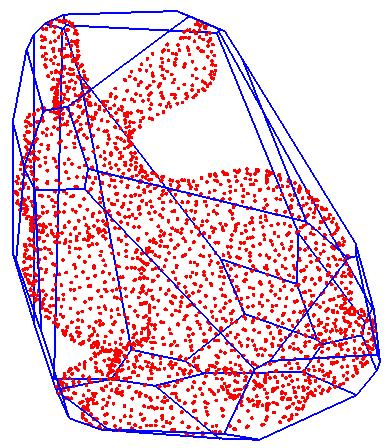
\includegraphics[width=0.25\textwidth]{bunny-34.png}}}
        \end{column}

       %\pgfputat{\pgfxy(7,-1.5)}{\pgfbox[left,top]{
       %  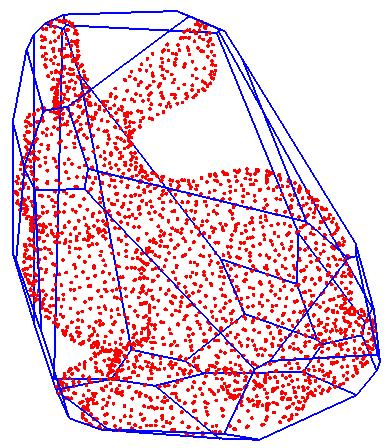
\includegraphics[width=0.25\textwidth]{bunny-34.png}
       %}}
        \begin{column}{0.4\textwidth}
        \begin{figure}
            %\pgfputat{\pgfxy(7,-1.5)}{\pgfbox[left,top]{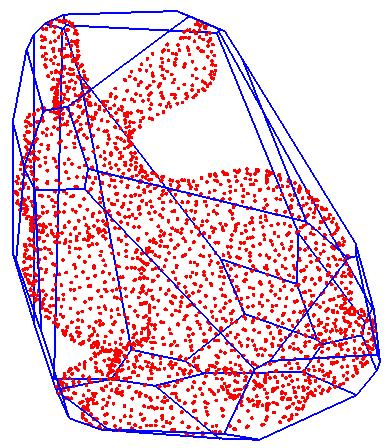
\includegraphics[width=0.8\textwidth]{bunny-34.png}}} %%cannot use caption for pgfputat
            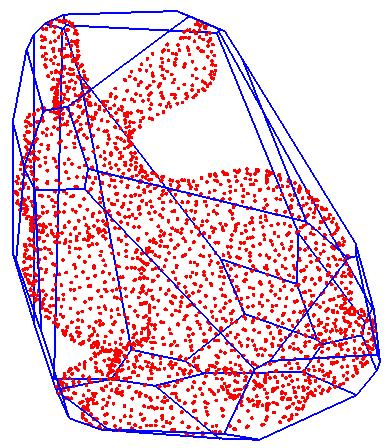
\includegraphics[width=0.8\textwidth]{bunny-34.png}
            \caption{34-CBP}
        \end{figure}
        \end{column}
      \end{columns}
    }

       \frame{
       \frametitle{算法流程}
       \begin{block}{构造$k$-CBP~算法流程图}
        \begin{figure}
        \centering
        %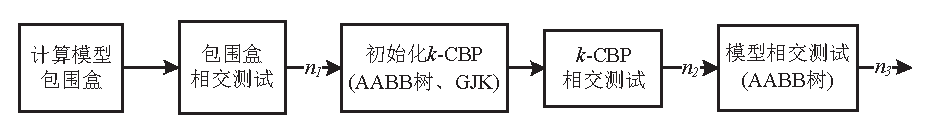
\includegraphics[width=4.0in]{figures/collision-detection-flowchart.eps}
        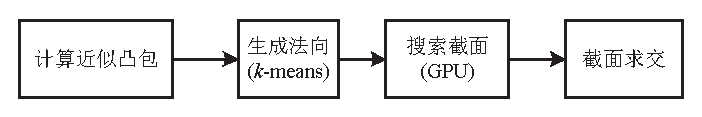
\includegraphics[width=4.0in]{kcbp-flowchart-x-aix.eps}
        %\caption{构造$k$-CBP~算法流程图}
        \label{lbl:kcbp-algorithm-flowchart}
        \end{figure}
     %   \hspace*{.1\linewidth}
     %   \begin{minipage}{\textwidth}
     %     \begin{exampleblock}{关键步骤}
     %     \begin{description}
     %        \item[定法向:]结合近似内凸包和~$k$-means~
     %        \item[搜截面:]GPU~中沿各法向搜索切点构造截面
     %        \item[求交点:]截面对偶映射求得交点
     %     \end{description}
     %   \end{exampleblock}
     % \end{minipage}
    \end{block}
    \begin{block}{关键步骤}
          \begin{description}
             \item[定法向:]结合近似内凸包和~$k$-means~
             \item[搜截面:]GPU~中沿各法向搜索切点构造截面
             \item[求交点:]截面对偶映射求得交点
          \end{description}
    \end{block}
    }

  \subsection{截面法向的生成}

    \frame{
        \frametitle{近似凸包的构造}
        \begin{figure}
        \vspace{-3mm}
        \subfloat[分组]
        {
           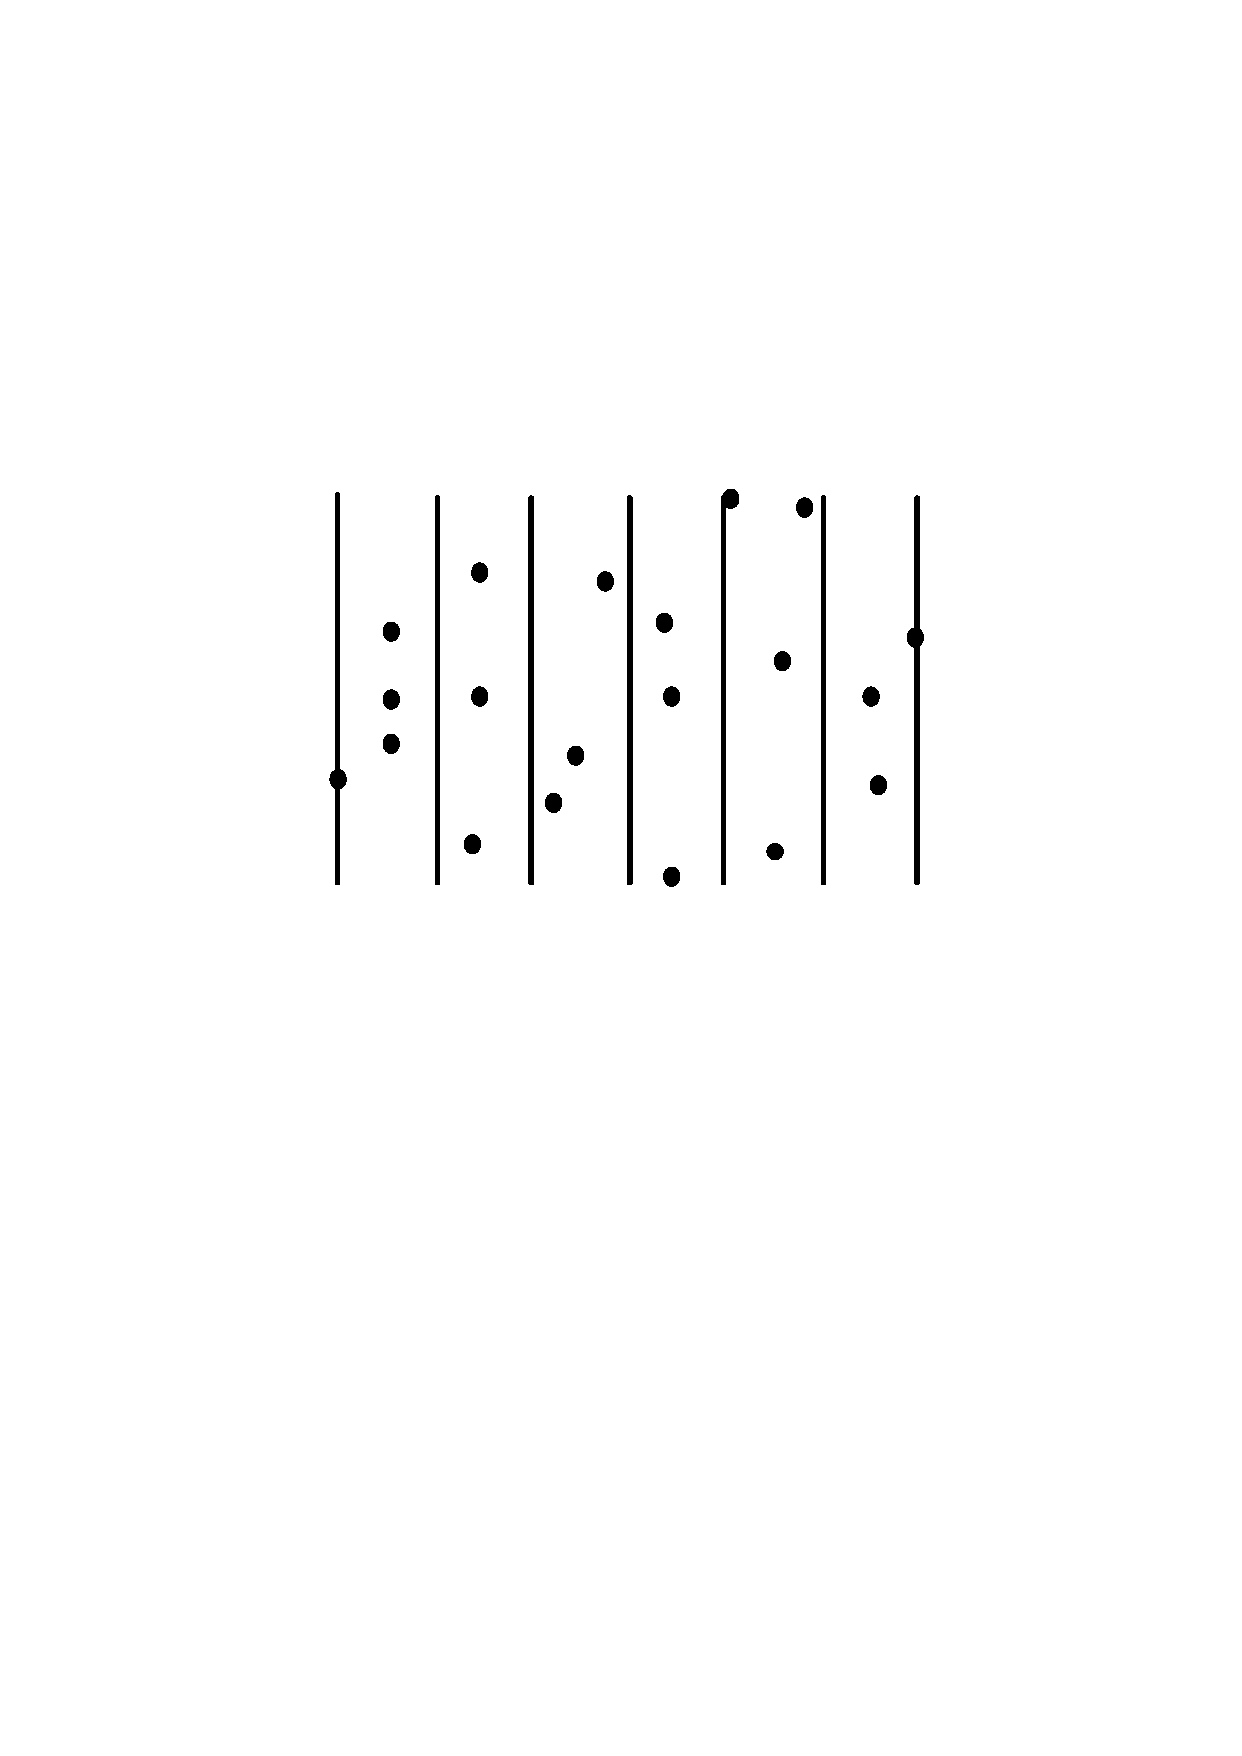
\includegraphics[width=0.28\textwidth]{figures/approximate-convexhull-step1.pdf}
        }\hspace{2mm}
        \subfloat[选极值点]
        {
            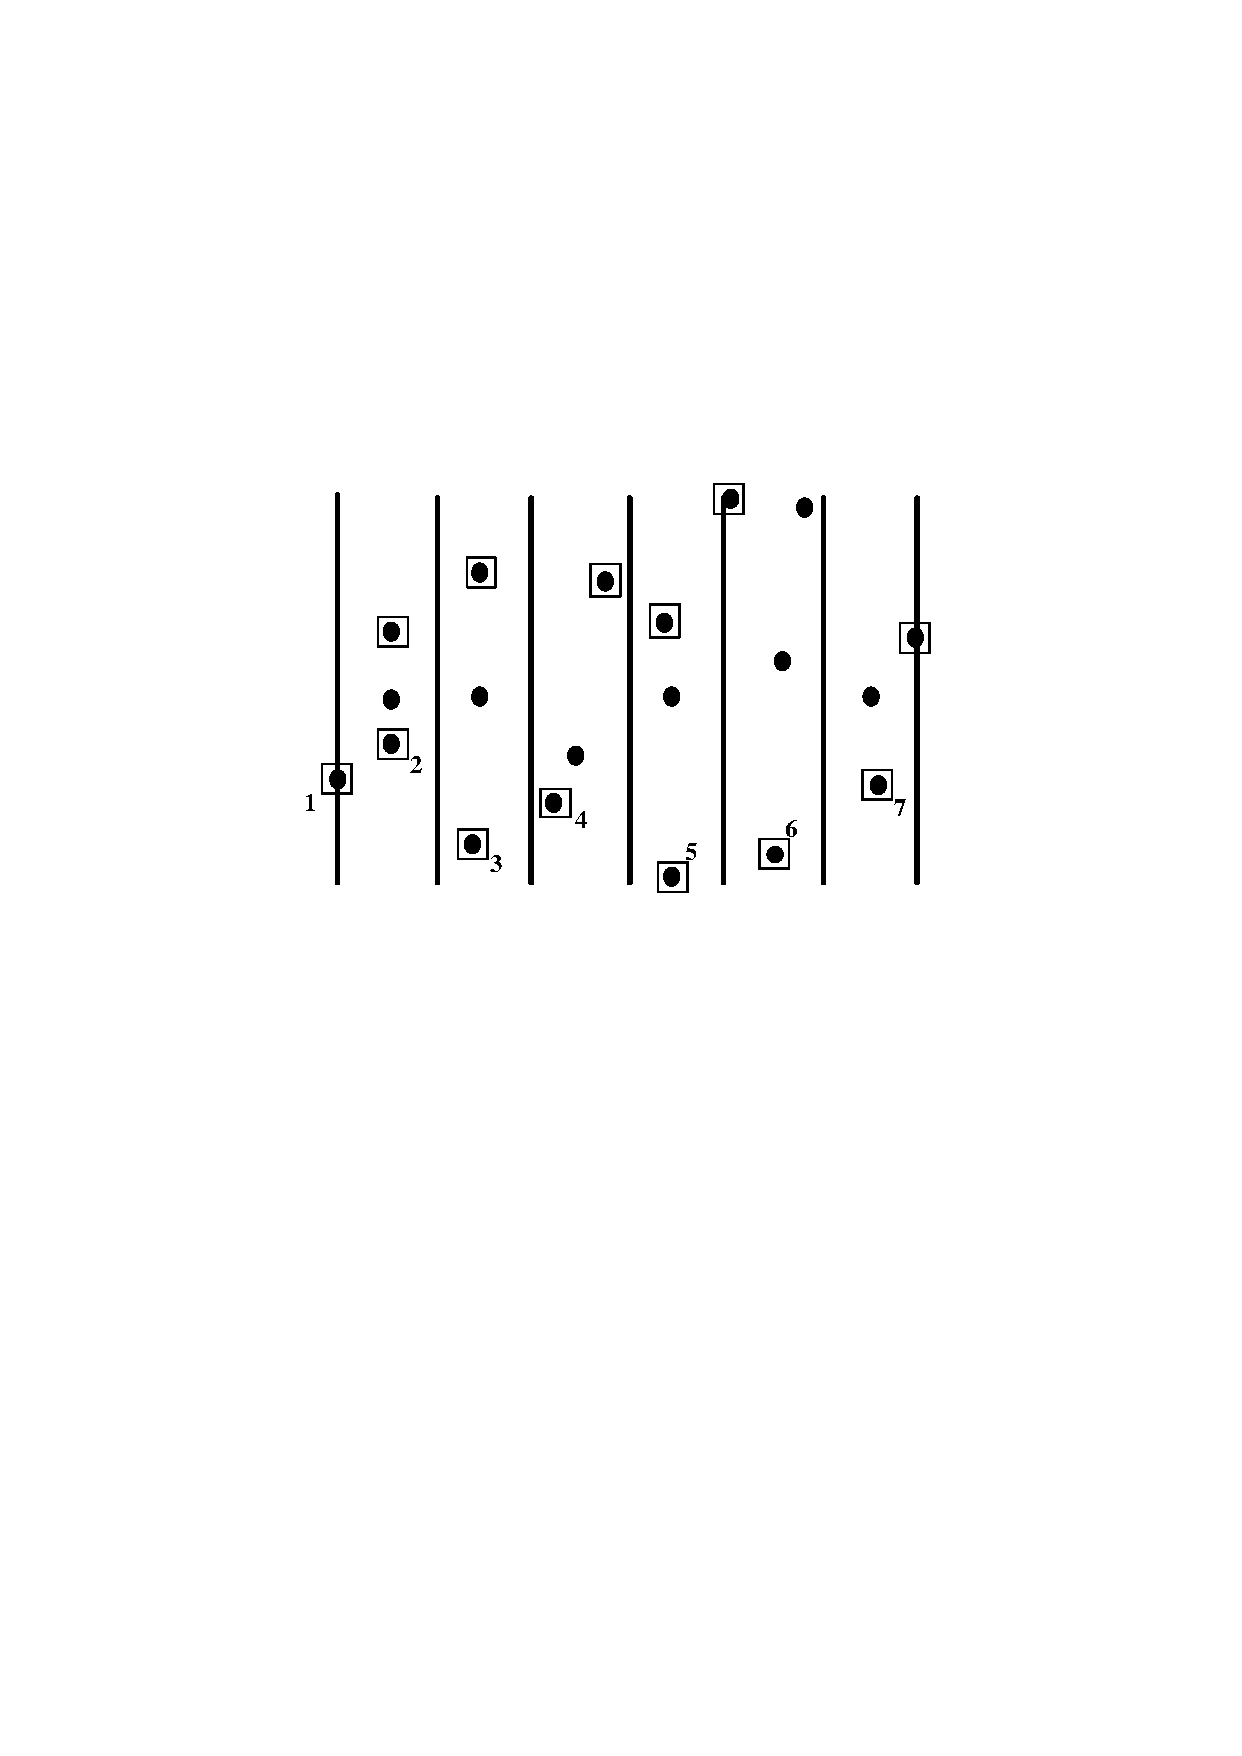
\includegraphics[width=0.28\textwidth]{figures/approximate-convexhull-step2.pdf}
        }\hspace{2mm}
        \subfloat[连线]
        {
           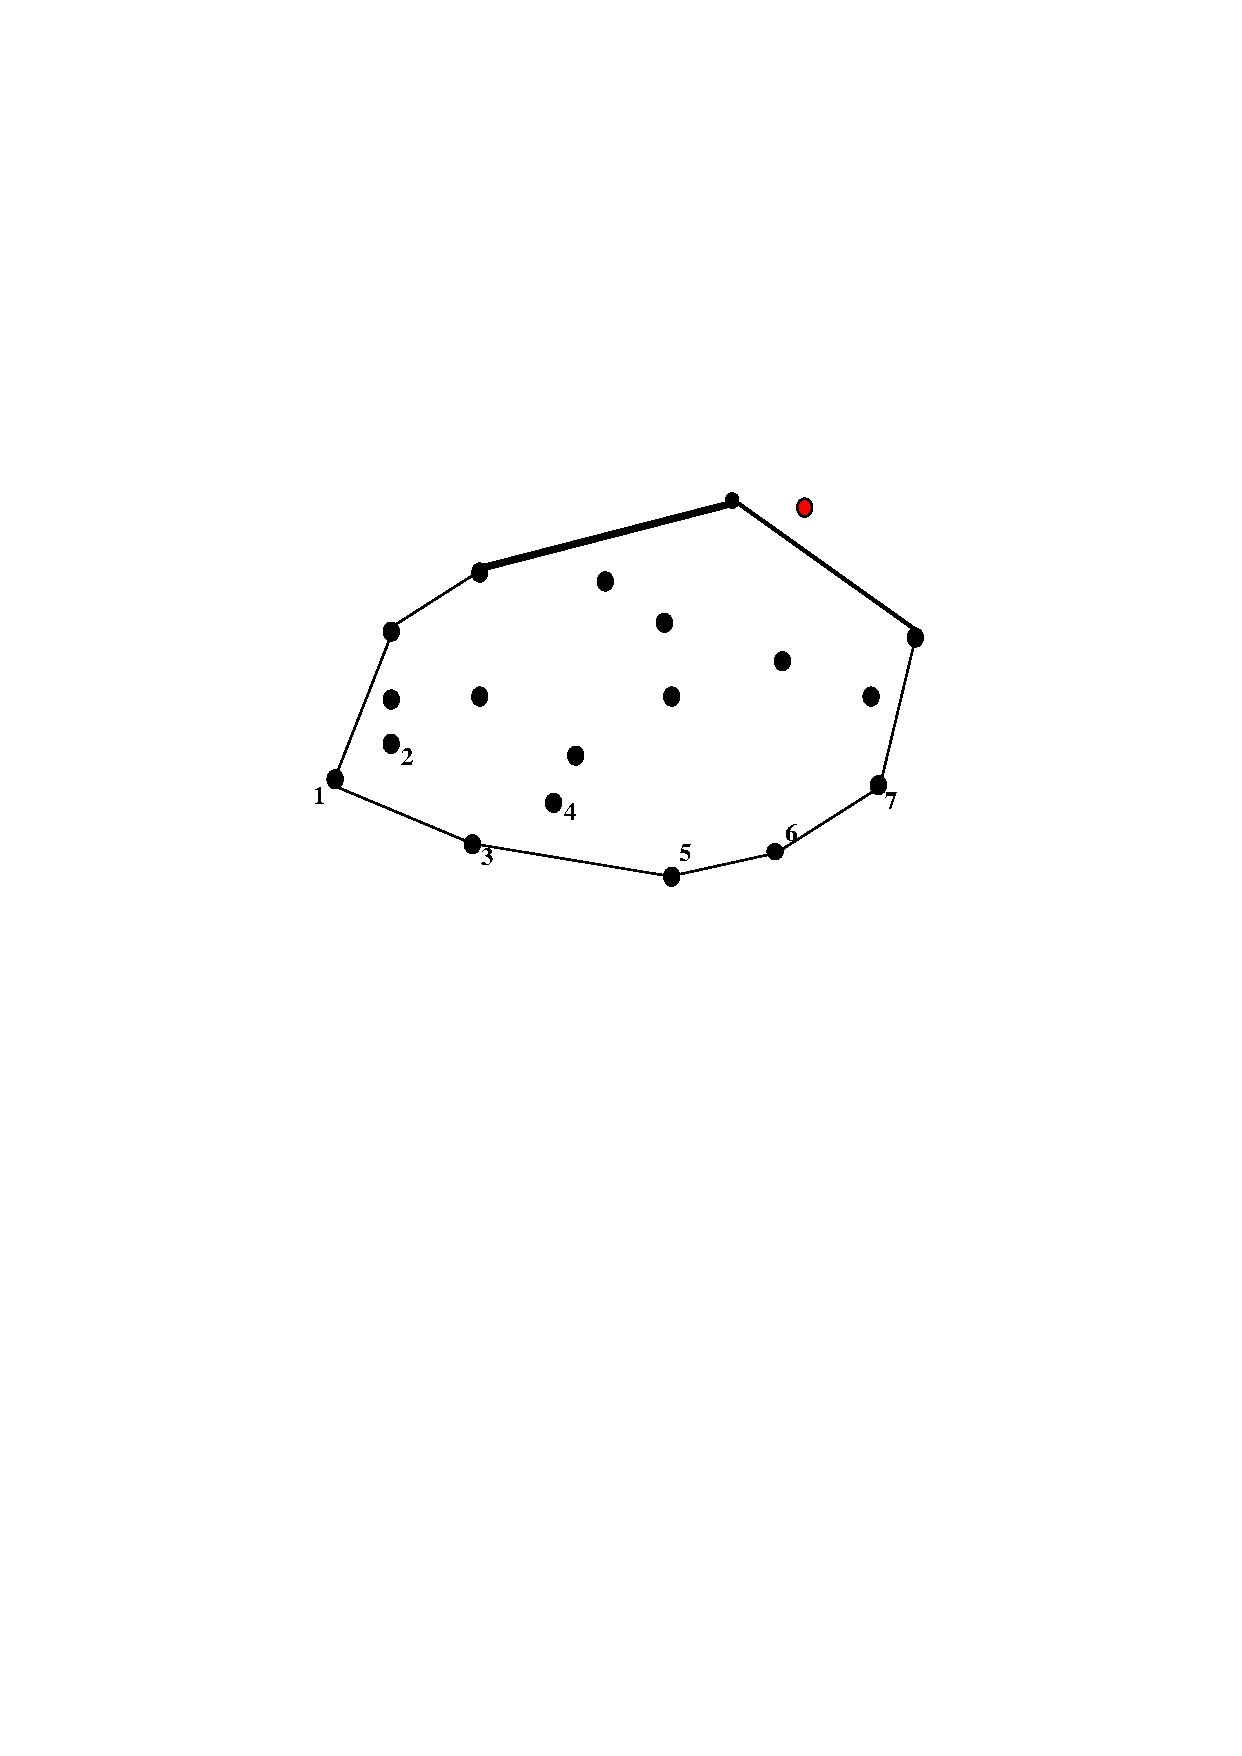
\includegraphics[width=0.28\textwidth]{figures/approximate-convexhull-step3.pdf}
        }
        \caption{二维近似内凸包的构造}
        \label{lbl:ach-2d}
        \end{figure}
        \vspace{-4mm}
        构造近似内凸包\cite{bentley1982approximation},算法复杂度为~$O(n+\xi)$,扩展到三维为~$O(n+\xi^2\log\xi)$,然后利用$k$-means 聚类。
    }
    \frame{
        \frametitle{$k$-means 聚类}
      \begin{figure}
        \vspace{-2mm}
        \subfloat[]
        {
           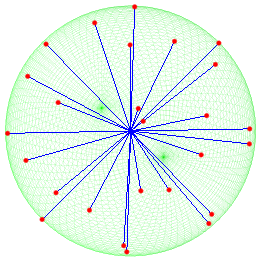
\includegraphics[width=0.28\textwidth]{kmeans-init-normals-26.png}
        }
        \subfloat[]
        {
            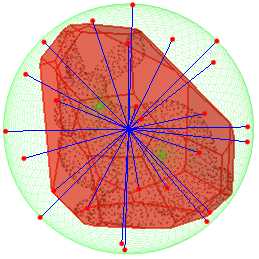
\includegraphics[width=0.28\textwidth]{kmeans-init-normals-26-for-bunny.png}
        }
        \subfloat[]
        {
           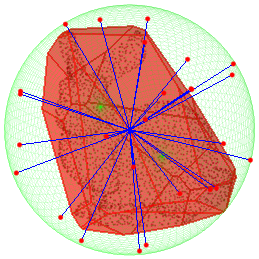
\includegraphics[width=0.28\textwidth]{kmeans-cluster-normals-26-for-bunny.png}
        }
        \vspace{-2mm}
        \caption{通过聚类确定法向}
        \label{lbl:gen-fixed-normals}
        \end{figure}
        %\begin{block}{聚类关键}
            \begin{description}
             \item[初始方向:]均匀分布;
             \item[聚类度量:]余弦;
             \item[中心更新:]
       中心点:$\bm{c_i}=\frac{\sum_{i=1}^{i=n} \omega_i \cdot \bm{n_i} } {\sum_{i=1}^{i=n} \omega_i}$,权重$\omega_i$为面片面积。
            \end{description}
       % \end{block}
    }

  \subsection{搜索截面}
    \frame{
    \frametitle{搜索截面}
    \begin{block}{截面=法向+点}
     法向已得,求投影点:对每个法向~$\bm{n_i}$,从输入模型的所有点中寻找最大投影值的点作为切点。
	时间复杂度为~$O(k\cdot n)$, 其中~$k$~为法向数量, $n$~为模型所含点数. 
   \end{block}
   \begin{block}{并行可行性}
	各法向的计算相互独立, 借助~GPU~并行加速。
	典型GPU并行平台:着色器(GLSL为例)和基于 GPU 的通用计算框架(CUDA为例)
	\end{block}
    }
    
    \frame{
    \frametitle{GLSL实现}
	     \begin{columns}[onlytextwidth]
     		 \begin{column}{0.5\textwidth}
		 \begin{figure}
	    		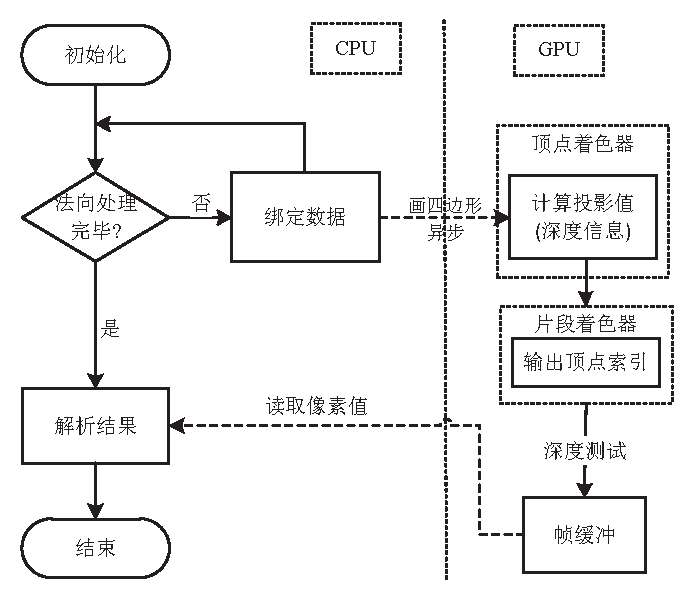
\includegraphics[width=\textwidth]{shader-z_buffer.eps}
	    		\caption{基于Z Buffer算法流程图}
		\end{figure}
	    	\end{column}
		
		\hspace{1em}
		
		 \begin{column}{0.5\textwidth}
		   	\begin{figure}
		 	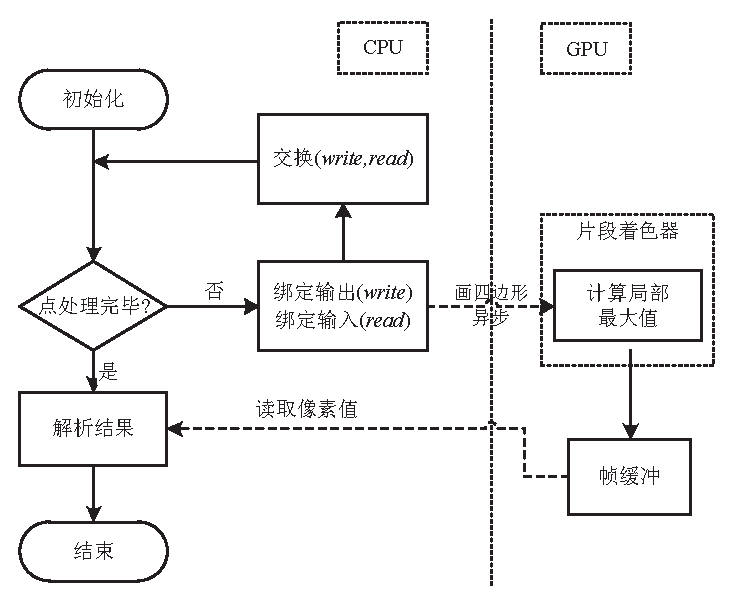
\includegraphics[width=\textwidth]{shader-rtt_pp.eps}
	    		\caption{基于乒乓技术算法流程图}
			\end{figure}	
	    	\end{column}
       	     \end{columns}
   }
    
    \begin{frame}
    \frametitle{CUDA实现}
	    \begin{figure}
	    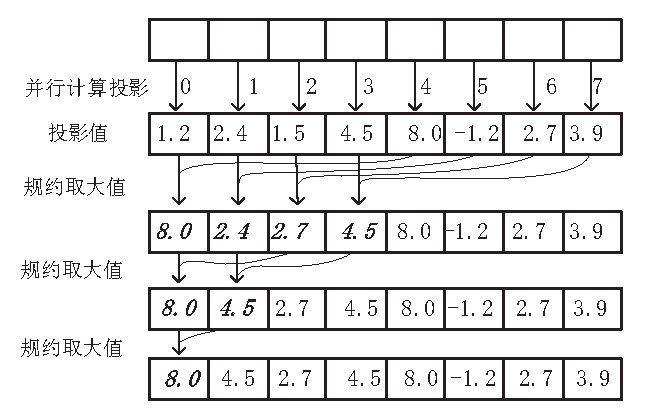
\includegraphics[width=2.5in]{gpureduction.eps}
	    \caption{并行规约求最大投影值}
	    \label{lbl:reduction-getmax}
	    \end{figure}
	    \vspace{-1.5em}
	    \small 
	    将输入点交给数量为~$t$~的线程计算点积得到投影值,
 线程~$i$~和~$i+t/2$~比较选取较大者,经~$\log_2t$~次比较可得最大值。OpenCL等并行计算框架类似。
    \end{frame}

        \frame{
    \frametitle{求交算法}
      \begin{block}{直接枚举}
      通过枚举所有每~3~个平面交于~1~点的情况,然后排除在平面外部的交点,剩下的构成~$k$-CBP~的顶点,时间复杂度为$O(k^3)$。
      \end{block}
      \begin{block}{对偶映射}
        法向~$\bm{n}(a,b,c)$~ + 平面上点~$\bm{p}(x_0,y_0,z_0)$ $\Rightarrow$ 平面方程~$ax + by + cz = ax_0 + by_0 + cz_0=d$, $d \neq 0$ \\
        对偶点为~$\bm{p'}(a/d, b/d, c/d)$,对~$k$~个映射点求凸包,凸包平面映射回原来的交点,时间复杂度为$O(k\log k)$。
      \end{block}
    }


  \subsection{实验与分析}

  %\subsubsection{凸包围多面体的生成速度}

    \frame{
      \frametitle{生成$k$-CBP的效率:GLSL实验结果}
      \begin{figure}[htbp] % use [htbp] to fix the position
        \vspace{-8mm}
      \subfloat %Apple模型(8118个点)
      {  
         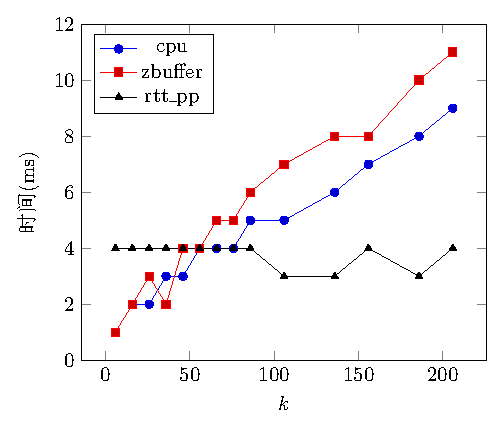
\includegraphics[width=\fourgraphicswidth\textwidth,page=1]{shadertime.pdf}
      }
      \subfloat % Buddha模型(31232个点)
      {  
          \includegraphics[width=\fourgraphicswidth\textwidth, page=2]{shadertime.pdf}
      }\vspace{-8mm}\linebreak %强制换行
        \vspace{-3mm}%
      \subfloat % Alice模型(224291个点)
      {  
         \includegraphics[width=\fourgraphicswidth\textwidth, page=3]{shadertime.pdf}
      }
      \subfloat % Bugatti模型(1010815个点)
      {  
         \includegraphics[width=\fourgraphicswidth\textwidth, page=4]{shadertime.pdf}
      }
      \caption{\tiny Apple(8k), Buddha(31k), Alice(224k), Bugatti(1011k)}
      \label{fig:chart:exps:shadertime}
      \end{figure}

      \note{
      从实验结果可以看出,当模型规模不大时,如图~\ref{fig:exp:shader:apple}~所示的含有8千多个点的~Apple~模型,
Z Buffer~算法和传统的~CPU~算法差别不是很大,因此在实际应用中当模型规模较小时可直接用~CPU~计算即可。
随着输入模型所含有点的数量规模的增加,CPU~和~GPU~运行时间之间的差距也越来越大。
当多面体面数增加即~$k$~的增大时,在~Z Buffer~算法中,需要更多的绘制次数,因此其运行时间也有所增加,而在基于乒乓技术的算法中,当点规模一定时,$k$~的变化对最后运行时间影响不明显,因此当较大的~$k$~时,这种算法更快。
      }
    }

    \frame{
      \frametitle{生成$k$-CBP的效率:CUDA实验结果}
        \begin{figure}
        \vspace{-8mm}
        \subfloat%[\tiny Budda(31232 points)]
        { 
           \includegraphics[width=0.35\textwidth,page=2]{figures/cudatime.pdf}
        }
        \subfloat%[\tiny Dinosaur(40277 points)]
        { 
            \includegraphics[width=0.35\textwidth, page=3]{figures/cudatime.pdf}
        }\vspace{-8mm}\linebreak %强制换行
        \vspace{-3mm}%
       \subfloat%[Alice(224291 points)]
        {
           \includegraphics[width=0.35\textwidth, page=4]{figures/cudatime.pdf}
        }
        \subfloat%[Bugatti(1010815 points)]
        {
           \includegraphics[width=0.35\textwidth, page=5]{figures/cudatime.pdf}
        }
        \caption{\tiny Budda(31k),Dinosaur(40k),Alice(224k), Bugatti(1011k)}
        \label{chart:exps:cputime}
        \end{figure}

        \note{
        图~\ref{chart:exps:cputime} 中横纵坐标分别代表多面体面数和运行时间, 其中虚线代表搜索截面的过程, 实线为构造凸包围多面体总体耗时. 当模型点数量较大时, 搜索截面的过程占据了算法绝大多数时间, 且随着凸包围多面体的面数~$k$~ 值增加而线性增长, 这与搜索截面时间复杂度($O(k\cdot n)$)一致, 截面求交过程的时间复杂度为$O(k\log k)$,
当点数量极大时, 实线虚线几乎重合即求交等步骤耗时相比整体算法而言几乎可忽略.
        }
    }

    \frame{
      \frametitle{生成$k$-CBP的效率:与文献\cite{karlsson2010parallel}算法对比}
        \vspace{-7mm}
        \begin{table} \tiny
        \caption{本文算法与文献\cite{karlsson2010parallel}算法对比}
        \begin{tabular}{p{1.5cm}<{\centering}ccc ccc} %p本身占一列
       \toprule[1pt]
        \multirow{2}{*}{$k$} & \multicolumn{3}{c}{Apple(8118 points)} & \multicolumn{3}{c}{~~~~~Bugatti(1010815 points)}\\
        %\cmidrule(lr){2-4}\cmidrule(lr){5-7}
        %\hline
        %\rowcolor[gray]{0.9} $k$ &
        ~&SSE(ms) & $k$-CBP(ms) &  Speedup &SSE(ms) & $k$-CBP(ms) &  Speedup \\
     \midrule[0.5pt]
        6 & 0.4 & 0.12  & 3.20     & 24.2 & 3.20  & 7.56 \\
        16 & 0.9 & 0.26  & 3.43    & 44.5 & 8.44  & 5.27 \\
        26 & 1.4 & 0.41  & 3.38    & 66.5 & 13.65  & 4.87 \\
        36 & 1.9 & 0.52  & 3.65    & 91.1 & 18.34  & 4.97 \\
        46 & 2.5 & 0.67  & 3.74    & 119.5 & 24.13  & 4.95 \\
        56 & 2.9 & 0.79  & 3.66    & 138.4 & 28.86  & 4.80 \\
        66 & 3.5 & 0.95  & 3.69    & 170.6 & 34.10  & 5.00 \\
        76 & 4.0 & 1.08  & 3.70      & 197.1 & 39.85  & 4.95 \\
        86 & 4.5 & 1.22  & 3.69    & 219.8 & 45.08  & 4.88 \\
        106 & 5.4 & 1.49  & 3.62   & 267.8 & 55.52  & 4.82 \\
        136 &  6.8 & 1.92  & 3.54  & 342.9 & 71.24  & 4.81 \\
        156 &  7.7 & 2.17  & 3.55  & 411.3 & 81.18  & 5.07 \\
        186 &  9.3 & 2.60  & 3.58  & 479.4 & 97.39  & 4.92 \\
        206 &  10.5 & 2.85  & 3.68 & 523.0 & 106.87  & 4.89  \\  
        \bottomrule[1pt]
        \end{tabular}
        \label{tab:exp:sse-time}
        \end{table}
        \vspace{-3mm}
        \scriptsize  当点数量较小时,能够提高~3-4~倍速度,模型变大,加速比更大,Bugatti~模型的提速达到~4$\sim$8~倍。
    }

  %\subsubsection{凸包围多面体的紧致程度}
   \frame{
        \frametitle{生成$k$-CBP的紧致程度:$k$-DOP v.s $k$-CBP }
        \begin{figure}
        \vspace{-8mm}
        \subfloat
        {  
           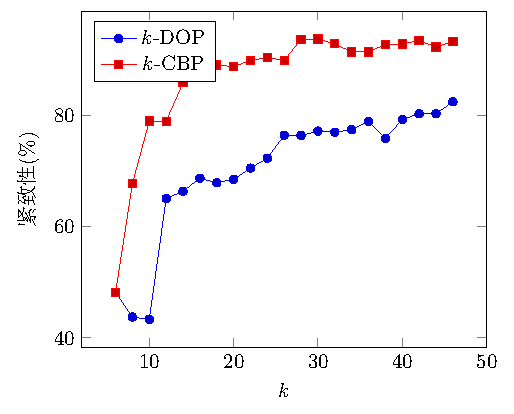
\includegraphics[width=0.35\textwidth,page=1]{figures/tightness.pdf}
        }
        \subfloat
        { 
            \includegraphics[width=0.35\textwidth, page=2]{figures/tightness.pdf}
        }\vspace{-8mm}\linebreak %强制换行
        \vspace{-3mm}%
       \subfloat%[Alice(224291 points)]
        { 
           \includegraphics[width=0.35\textwidth, page=3]{figures/tightness.pdf}
        }
        \subfloat%[Bugatti(1010815 points)]
        {
           \includegraphics[width=0.35\textwidth, page=4]{figures/tightness.pdf}
        }
        \caption{紧致程度对比: \tiny Apple(8k), Budda(31k), Dinosaur(40k), Alice(224k)}
        \label{chart:exps:tightness}
        \end{figure}
        \vspace{-3mm}
        \scriptsize \centering 较~$k$-DOP~提升 10\% $\sim$ 40\%,下图可视化结果。
    }
    \frame{
      \frametitle{生成$k$-CBP的紧致程度:$k$-DOP v.s $k$-CBP }
      \hspace{3em}
      \vspace{-3em}
      \begin{figure}[H] 
        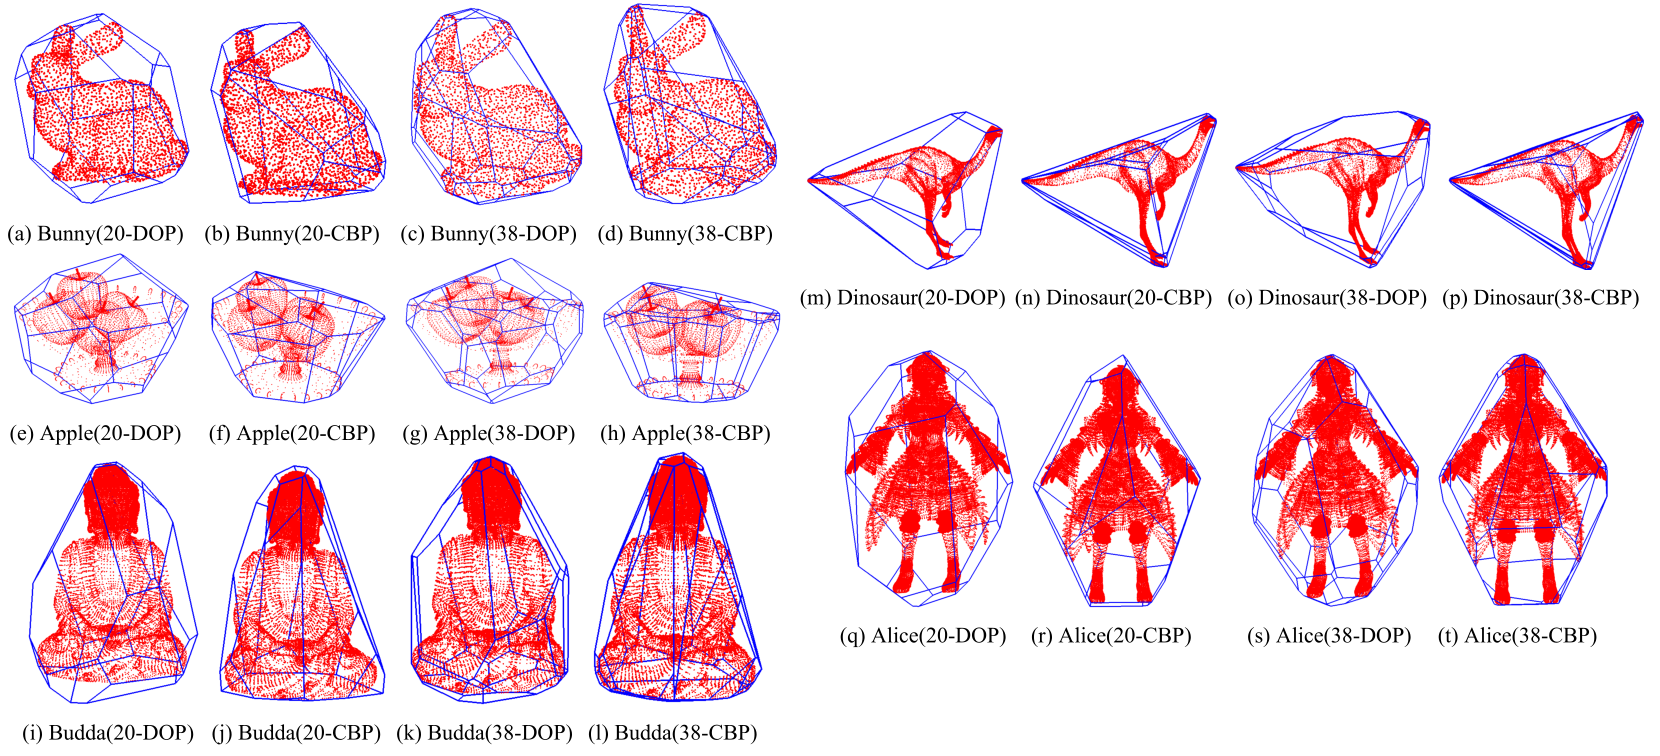
\includegraphics[width=1.05\textwidth]{kCBP-KDOP.png}
      \caption{~$k$-CBP~与~$k$-DOP~对比}
      \label{fig:kdop:kcbp:ui}
      \end{figure}
    }

    \frame{
        \frametitle{生成$k$-CBP的紧致程度:$k$-DOP v.s 凸包 }
       % \begin{block}{结果}
        \begin{table}
        \scriptsize
        \caption{\label{tab:exp:cgal}$k$-CBP~与~QuickHull~凸包算法比较}
         \begin{tabular}{lcccccl}
          \toprule
          Model & f(CHull)& f($k$-CBP) & $\tau$ ($k$-CBP) & t(CHull(ms)) & t($k$-CBP(ms))\\
          \midrule
          Apple	& 499 & 30 & 93.67\% & 5.5 & 1.30\\ % apple3  自己电脑跑的数据, 之前是用的chengxianyu的电脑.
          Budda	& 1608 & 46 & 92.39\% & 21.3 & 2.86 \\ %  1.0+0.86+1
          Dinosaur	& 1240 & 44 & 93.34\% & 22.6 & 1.99 \\  % 1.0+0.98+0.1
          Alice	& 1332 & 44 & 93.92\% & 85.8 & 8.47\\ % 2+6.48
          Bugatti & 24654 & 44 & 95.06\% & 688.7 & 25.41\\
          \bottomrule
         \end{tabular}
         \vspace{-2mm}
        \end{table}
       % \end{block}
        \begin{block}{结论}
        \scriptsize 与凸包相比,本文算法在大大简化包围体平面数量的同时能保持较好的紧致程度(Bugatti 凸包面的0.17\%的达到95.06\%紧致程度,构造速度快27倍),下图为可视化结果。
        \end{block}
    }

    \frame{
        \frametitle{生成$k$-CBP的紧致程度:$k$-DOP v.s 凸包}
        \begin{figure}
        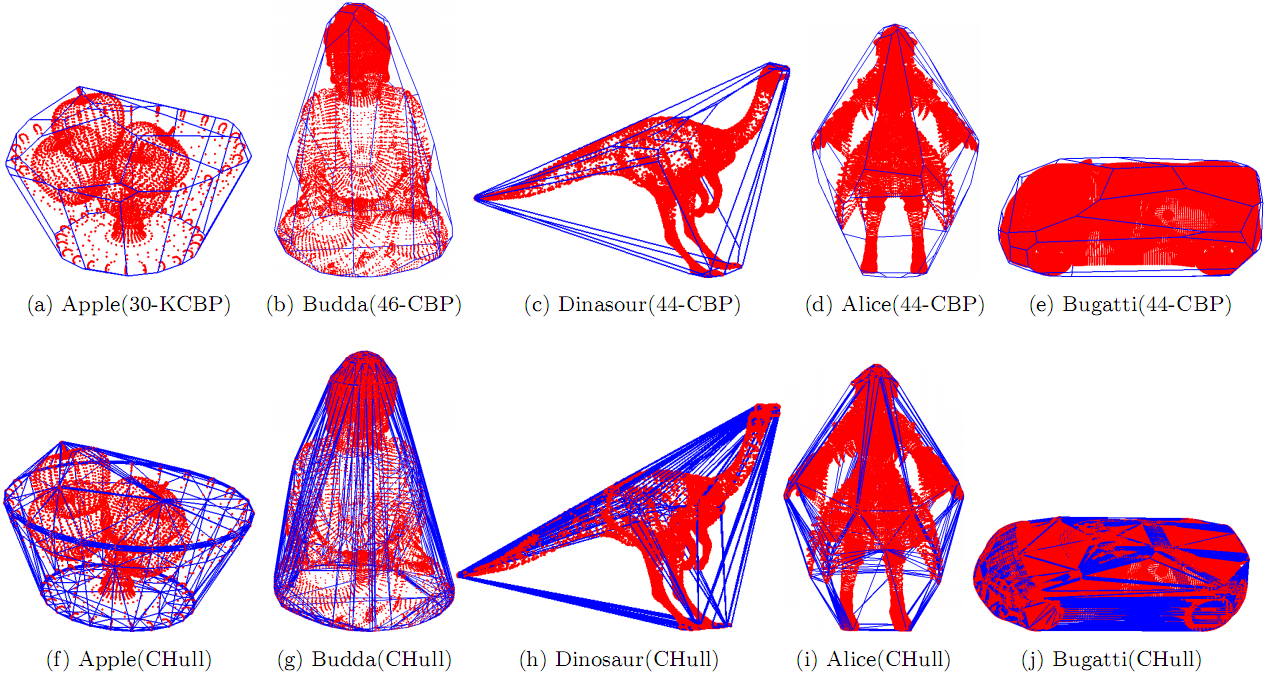
\includegraphics[width=4.0in]{figures/kcbp-convexhull.png}
        \caption{$k$-CBP~与凸包对比}
        \label{pic:exps:ch-kcbp}
        \end{figure}
    }

      \section{基于$k$-CBP~的碰撞检测算法}
    
      \subsection{$k$-CBP~间的相交测试}
      \begin{frame}
        \frametitle{}
        \begin{block}{AABB树法}
          将生成的$k$-CBP视为普通的三角网格,实现简单,适用于模型较小的静止碰撞检测场景
        \end{block}
        \begin{block}{GJK法}
          计算凸多面体之间的最近距离的~GJK~算法。\\
          Minkowski~差,即~$\mathbb{A} - \mathbb{B} = \{ \bm{a} - \bm{b} | \bm{a} \in \mathbb{A}, \bm{b} \in \mathbb{B}\} $。
GJK~算法的核心基础在于若两个凸多边相交,则凸多边形顶点的~Minkowski~差所围成的多边形必包含原点,因为若~$\mathbb{A}$~和
~$\mathbb{B}$~相交即~$\mathbb{A}$~和~$\mathbb{B}$~必含有公共交集,
即至少含有一点同时属于~$\mathbb{A}$~和~$\mathbb{B}$~,该点的~Minkowski~差即为原点~$\bm{O}(0, 0)$。
        \end{block}
      \end{frame}

      \begin{frame}
        \frametitle{二维~GJK~算法示例}
        \begin{figure}[htbp]
        \subfloat[相交]{
          \includegraphics[width=.48\textwidth]{gjkIntersection.tikz}
        } 
        \subfloat[不相交]{
          \includegraphics[width=.48\textwidth]{gjkNonIntersection.tikz}
        }
        \end{figure}
      \end{frame}
      
      \subsection{三角网格间的相交测试}
      
      \subsection{基于$k$-CBP~的碰撞检测算法}

    \frame{
        \begin{figure}
        \centering
        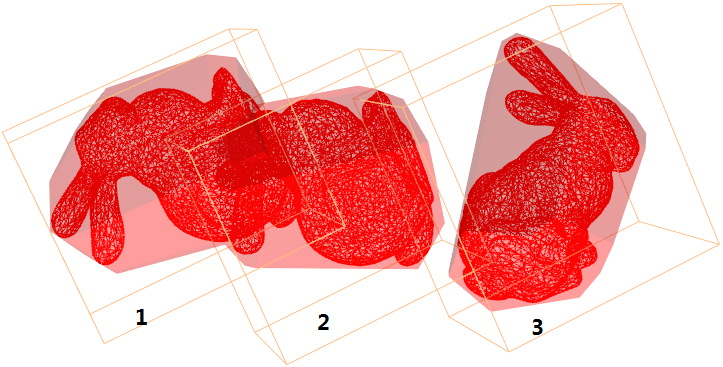
\includegraphics[width=3in]{figures/bunny-box-kcbp-collsion-detection-example.png}
        \caption{~$k-$CBP~应用于碰撞检测示例}
        %\centerline{\bahao\bf 图 10\quad ~$k-$CBP~应用于碰撞检测示例}
        %\centerline{\footnotesize {\bf Figure 10}\quad  Example of collision detection using $k$-CBP}
        \label{lbl:bunny-box-kcbp-collsion-detection-example}
        \end{figure}

        \small 图中模型~1~与~2、2~与~3~的包围盒分别相交, 而其~$16$-CBP~仅~1~与~2~相交, 实际模型仅~1~与~2~相交. 不同数量的模型(模型位置和旋转角度随机生成)测试结果如下表所示.
    }

    \subsection{实验结果及分析}

    \frame{
        \begin{table}
        \tiny
        \centering
         \caption{\label{tab:exp:box:kcbp:collsiondetection}$k$-CBP~和包围盒应用于碰撞检测结果对比}
        % \centerline{\zihao{-5}\bf \small 表4\quad }
        %\centerline{\footnotesize{\bf Table 4}\quad Comparison of result of collision detection between $k$-CBP and bounding box}
        %\vspace{3mm}{\zihao{6}\footnotesize
        %\begin{center}\belowrulesep=0pt\renewcommand{\arraystretch}{1.3} \doublerulesep 0.4pt \tabcolsep 10pt
         \begin{tabular}{lccccccl}
          \toprule
          n& c(Box) & c($16$-CBP) &  t(Box) & t($16$-CBP) & r(Box) & r($k$-CBP) & n(Model) \\
          \midrule
           10 & 0.1 & 1.8 &    26.0  & 0.1    & 0.00 \% &  100.00\% & 0\\
           30 & 0.2 & 2.9 &   134.0  & 70.0   & 45.45\% & 83.33\% & 5\\
           50 & 0.5 & 4.8 &   506.0  & 255.2  & 46.34\% & 86.36\% & 19 \\
           70 & 0.4 & 4.8 &   901.1  & 492.5  & 44.16\% & 80.95\% & 34 \\
           90 & 0.7 & 5.7 &  1324.0  & 734.7  & 41.82\% & 73.02\% & 46 \\
          100 & 0.7 & 7.8 &  1481.0  & 870.7  & 43.31\% & 75.34\% & 55 \\
          150 & 1.0 & 9.8 &  4153.1  & 2473.0 & 42.98\% & 70.75\% & 150 \\
          200 & 1.6 & 12.8 & 8049.3  & 4430.9 & 41.02\% & 71.32\% & 281 \\
          \bottomrule
         \end{tabular}
         % \end{center}}\vspace{-2mm}
        \end{table}
        \small 其中~r(Box), r($16$-CBP)分别表示包围盒、16-CBP~的命中率即用实际模型相交的数量除以包围体检测出来相交的数量. 模型和凸包围多面体是否相交都采用了普通~AABB~ 树的方式进行判断.
    }

    \section{主要参考文献}
    \frame[t,allowframebreaks]{
      \frametitle{\secname}
    \scriptsize
    \printbibliography
    }
    
    
    \section{感谢}
    \frame{
      \frametitle{\secname}
      导师、学院
    }

    \section{FAQ}
    \frame{
      \frametitle{\secname}
       Thank you!
    }





\end{document}

